%=======================================================================
% Escrevendo o Texto
%=======================================================================
\chapter{API de Gestão de Noticias}

Para este trabalho, foram desenvolvidas duas APIs de cadastro de notícias: uma utilizando Java com o framework Spring Boot, seguindo o paradigma orientado a objetos, e outra em Clojure, baseada no paradigma funcional. O objetivo dessa implementação é enriquecer o contexto do estudo, fornecendo um exemplo prático que permita a comparação entre os dois paradigmas. Nessa implementação, não foram priorizados aspectos como segurança da informação ou arquitetura avançada de software, pois o foco principal do trabalho está nos elementos específicos de cada paradigma.


\subsection{Descrição do sistema}

O sistema desenvolvido para este trabalho consiste em duas APIs de gestão de notícias, implementadas com diferentes paradigmas de programação: a primeira em Java utilizando o framework Spring Boot (paradigma orientado a objetos), e a segunda em Clojure (paradigma funcional). Ambas compartilham funcionalidades centrais semelhantes, mas foram desenvolvidas com abordagens distintas para permitir uma análise prática e comparativa entre os paradigmas.

\subsection{Funcionalidades Comuns}

Ambas as APIs oferecem funcionalidades relacionadas à gestão de notícias, com suporte para autenticação de usuários, cadastro, edição, exclusão e interação com notícias. Além disso, as APIs permitem listar usuários e interagir com as notícias através de curtidas. Apesar de implementações específicas variarem, as regras de negócio fundamentais seguem a mesma lógica:

\subsubsection{Autenticação de Usuário}

\begin{itemize}
    \item Os usuários podem logar através de suas credenciais (e-mail e senha).
\end{itemize}

\subsubsection{Cadastro e Gestão de Notícias}
\begin{itemize}
    \item As APIs oferecem a possibilidade de salvar notícias, buscando informações de fontes externas e armazenando-as no banco de dados.
    \item As notícias podem ser editadas ou excluídas por usuários com permissões administrativas.
\end{itemize}

\subsubsection{Interação com Notícias}
\begin{itemize}
    \item Os usuários podem "curtir" notícias, incrementando um contador de curtidas.
\end{itemize}

\subsubsection{Listagem de Usuários}
\begin{itemize}
    \item Administradores têm acesso a uma listagem completa de usuários cadastrados no sistema.
\end{itemize}

\subsection{Regras de Negócio}
As principais regras de negócio incluem:
\begin{itemize}
    \item Apenas administradores podem editar ou excluir notícias.
    \item As notícias são salvas com base em dados recuperados de uma API externa.
    \item O contador de curtidas é atualizado por meio de ações dos usuários.
\end{itemize}

\subsection{Estrutura e Implementação da API em Java}
A API em Java foi estruturada com o Spring Boot, utilizando práticas típicas do paradigma orientado a objetos, como encapsulamento e abstração. As principais classes estão organizadas em pacotes para controle, serviços e domínio. A arquitetura segue o padrão MVC (Model-View-Controller), com camadas bem definidas:
\begin{itemize}
    \item \textbf{Controladores}: Gerenciam as rotas e as requisições HTTP.
    \item \textbf{Serviços}: Implementam a lógica de negócios.
    \item \textbf{Modelos de Domínio}: Representam os objetos persistidos no banco de dados.
\end{itemize}

Os endpoints são claramente definidos, com suporte para operações como login (\texttt{/users/login}), salvar notícias (\texttt{/news/save}), editar (\texttt{/news/edit}) e excluir notícias (\texttt{/news/delete}).

\subsection{Estrutura e Implementação da API em Clojure}
A API em Clojure segue uma abordagem funcional, com ênfase em imutabilidade e funções puras. A organização do código é funcionalmente modular, com arquivos separados para lógica de negócios (\texttt{logics.clj}), configuração de infraestrutura (\texttt{infraConfigs.clj}) e controle de rotas (\texttt{controllers.clj}).

A API prioriza simplicidade e foco no estado funcional. Os endpoints refletem a mesma funcionalidade da API em Java, mas com uma implementação que evita efeitos colaterais e utiliza estruturas de dados imutáveis.

\subsection{Considerações sobre o Banco de Dados}
Ambas as APIs utilizam o mesmo banco de dados relacional, o PostgreSQL, usando a ferramenta Supabase, que permite interagir com as tabelas como uma API REST:
\begin{itemize}
    \item \textbf{Usuários}:
    \begin{itemize}
        \item Inclui campos como \texttt{id}, \texttt{nome}, \texttt{email}, \texttt{senha} e \texttt{isadmin} (indicador de privilégio administrativo).
    \end{itemize}
    \item \textbf{Notícias}:
    \begin{itemize}
        \item Inclui campos como \texttt{id}, \texttt{title}, \texttt{abstract}, \texttt{url}, \texttt{published\_date}, \texttt{source}, \texttt{likes} e \texttt{created\_at}.
    \end{itemize}
\end{itemize}

A API em Java, orientada a objetos, utiliza práticas como herança e classes para organizar o código, enquanto a API em Clojure adota um paradigma declarativo e funcional, evitando estados mutáveis e promovendo reutilização através de funções puras.

Essa descrição detalhada das APIs desenvolvidas permite contextualizar as implementações e enfatizar suas diferenças paradigmáticas, destacando como cada abordagem impacta a clareza do código, a manutenção e a escalabilidade do sistema.


\subsection{Diagramação}

\subsubsection{Diagrama de Sequência}

O diagrama de sequência descreve o fluxo de interação entre os atores e o sistema para login de usuários e recuperação de notícias. Ele destaca os seguintes elementos:
\begin{itemize}
    \item \textbf{Login:} Um ator solicita a login enviando suas credenciais para o sistema.
    \item \textbf{News (notícias):} Após a autenticação, o sistema permite ao ator executar operações relacionadas à gestão de notícias, como a obtenção de uma lista de notícias.
    \item \textbf{Fluxo:} A sequência de mensagens reflete a troca de informações entre o usuário e os componentes do sistema.
\end{itemize}
Este diagrama ilustra como os componentes interagem em tempo real para garantir um login bem-sucedida e o acesso às notícias.

\begin{figure} [H]
    \centering
    \caption{Diagrama de Sequencia}
    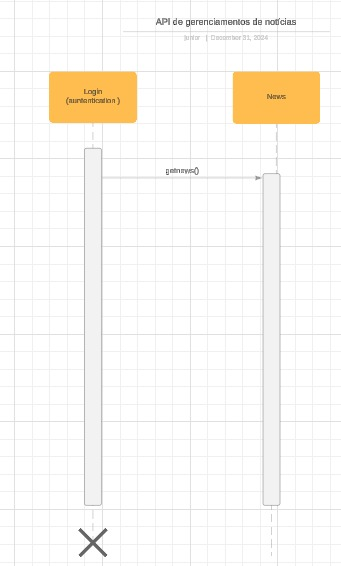
\includegraphics[width=0.5\linewidth]{imagens/sequencia diagrama.jpeg}
    \caption*{\textbf{Fonte:} Elaborado pelo autor usando Lucidchart.}
    \label{fig:enter-label}
\end{figure}

\subsubsection{Diagrama de Classes}

O diagrama de classes representa a estrutura lógica do sistema, identificando as principais entidades e suas relações:
\begin{itemize}
    \item \textbf{Administrador:} É uma subclasse de usuário com permissões adicionais para criar, editar e excluir notícias.
    \item \textbf{Usuário:} Entidade principal que representa qualquer pessoa autenticada no sistema, com funcionalidades como listar notícias e interagir (curtir ou descurtir).
    \item \textbf{Login:} Responsável pela entrada de usuários, vinculada à entidade de usuário.
    \item \textbf{Notícia:} Armazena informações sobre o conteúdo, autor, data de publicação, curtidas e outras propriedades relacionadas às notícias.
\end{itemize}
O diagrama também destaca a herança entre as classes \texttt{Administrador} e \texttt{Usuário}, indicando que administradores possuem todos os atributos e métodos de usuários, além de funcionalidades adicionais.


\begin{figure} [H]
    \centering
    \caption{Diagrama de Classe}
    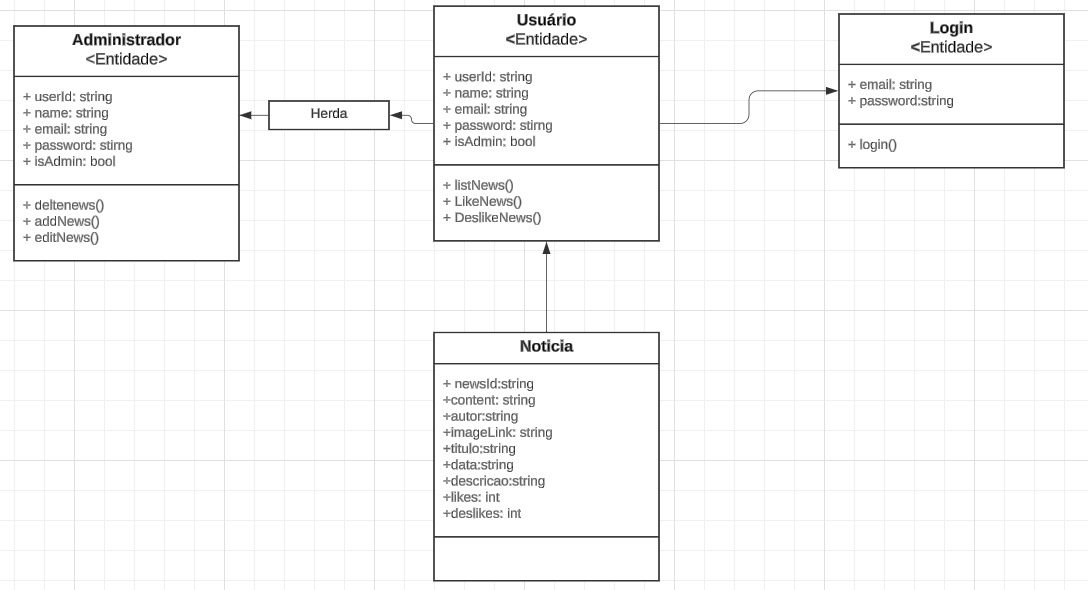
\includegraphics[width=0.5\linewidth]{imagens/diagram de objeto.jpeg}
    \caption*{\textbf{Fonte:} Elaborado pelo autor usando Lucidchart.}
    \label{fig:enter-label}
\end{figure}

\subsubsection{Diagrama de Caso de Uso}

O diagrama de caso de uso detalha as funcionalidades disponíveis para os diferentes atores do sistema:
\begin{itemize}
    \item \textbf{Usuário:} Pode listar notícias e interagir com elas (curtir ou descurtir).
    \item \textbf{Administrador:} Além das funcionalidades do usuário, pode criar, editar e excluir notícias. Essas ações estão associadas às permissões administrativas.
    \item \textbf{Sistema:} O sistema organiza essas interações para garantir que cada ator execute apenas as ações permitidas.
\end{itemize}
Este diagrama enfatiza a separação clara de responsabilidades entre os atores e a funcionalidade do sistema.



\begin{figure} [H]
    \centering
    \caption{Diagrama de Caso de Uso}
    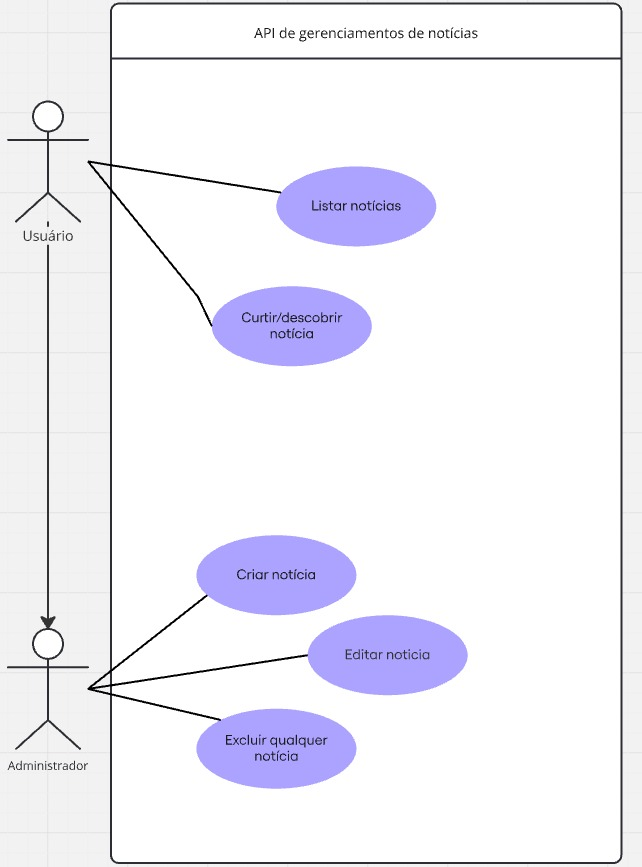
\includegraphics[width=0.5\linewidth]{imagens/diagram de caso de uso.jpeg}
    \caption*{\textbf{Fonte:} Elaborado pelo autor usando Miro.}
    \label{fig:enter-label}
\end{figure}



\chapter{Conceitos Funcionais}

Neste capítulo, exploramos os principais conceitos que fundamentam o paradigma de programação funcional. Esses conceitos são essenciais para compreender a abordagem funcional em comparação com paradigmas imperativos, como a programação orientada a objetos. Além de uma explicação teórica, são apresentados exemplos práticos em Clojure, uma linguagem funcional que foi utilizada no desenvolvimento deste trabalho.


\subsection{Imutabilidade}

A imutabilidade é um dos pilares da programação funcional (\citeonline{Higginbotham15}). Objetos imutáveis não podem ser alterados após sua criação. Isso reduz efeitos colaterais, melhora a previsibilidade do código e facilita a depuração. aplicar os conceitos em programas orientados objetos pode ser de grande benefício para esse software em questão.

\begin{tcolorbox}[colback=gray!5!white, colframe=gray!75!black, title={Quadro 7 - Imutabilidade}]
\begin{lstlisting}[language=Lisp]

(def lista-original [1 2 3])
(def lista-nova (conj lista-original 4)) ; Adiciona 4 sem modificar a lista original

;; Resultado:
;; lista-original => [1 2 3]
;; lista-nova => [1 2 3 4]

\end{lstlisting}
\caption{Exemplo de imutabilidade na linguagem Clojure.}
\end{tcolorbox}

A imutabilidade facilita o desenvolvimento de sistemas concorrentes, pois elimina a necessidade de controle de acesso simultâneo a dados compartilhados. Mas por que devemos nos preocupar com a imutabilidade em nossos códigos?
Os fabricantes de chips já atingiram os limites físicos da miniaturização de transistores. Como consequência, os "ticks" de clock das CPUs não aumentaram desde 2004. A estratégia atual para melhorar o desempenho está no uso de processadores multicore. No entanto, rotinas que compartilham estado mutável não podem ser executadas paralelamente em múltiplos núcleos de forma segura, enquanto a imutabilidade garante a segurança entre threads.
Além disso, a reatribuição de variáveis pode complicar a depuração de erros. Para reproduzir um bug complexo, é necessário compreender a sequência de cálculos que levou ao problema. Alterar variáveis durante a execução pode descartar essa sequência, tornando a análise de falhas mais difícil.


\subsubsection*{Como evitar mutações?}
Sempre que precisar modelar uma mudança de estado, você passa o valor anterior para uma função que retorna um novo valor. Não mude o valor antigo, apenas retorne um novo.

A API desenvolvida neste trabalho apresenta um exemplo simplificado para salvar notícias no banco de dados:

\begin{tcolorbox}[colback=gray!5!white, colframe=gray!75!black, title={Quadro 8 - Integração com Supabase}]
\begin{lstlisting}[language=Lisp]
(let [url "https://supabase.co/rest/v1/noticias"
      headers {"Authorization" (str "Bearer " token)
               "Content-Type" "application/json"}
  (client/post url {:headers headers :form-params body :as :json}))
\end{lstlisting}
\caption{Exemplo simplificado de salvamento de notícias no banco Supabase.}
\end{tcolorbox}

O mapa body é criado como uma nova estrutura de dados para cada notícia iterada, sem alterar o objeto original (noticia). Essa prática evita mudanças inesperadas no estado dos dados, garantindo maior previsibilidade e segurança no sistema. Objetos, sendo referências, podem gerar situações de estados pouco claros se suas propriedades forem alteradas. Ao evitar mudanças nos objetos após sua construção, conseguimos um código mais simples de entender, testar e depurar. Essa abordagem reflete os benefícios da imutabilidade, como a eliminação de efeitos colaterais e a simplificação do fluxo de dados. Além disso, ela promove um design alinhado aos princípios funcionais, especialmente em operações críticas, como interações com bancos de dados externos, resultando em sistemas mais robustos e previsíveis.

\subsection{lazy Evaluation}

A avaliação preguiçosa, ou lazy evaluation, é um conceito importante na programação funcional. Esse paradigma permite que valores sejam calculados apenas quando realmente necessários, diferentemente da avaliação estrita, onde todas as expressões são resolvidas imediatamente. Essa técnica otimiza o uso de recursos, permitindo o processamento eficiente de grandes coleções de dados ou até mesmo de coleções infinitas.

No contexto da API desenvolvida em Clojure, a avaliação preguiçosa é ilustrada pela manipulação de uma sequência infinita com o uso da função `range` combinada com `take`. Isso garante que apenas os valores estritamente necessários sejam calculados, otimizando o uso de memória e processamento. 

\begin{tcolorbox}[colback=gray!5!white, colframe=gray!75!black, title={Quadro 9 - Exemplo de Lazy Evaluation em Clojure}]
\begin{lstlisting}[language=Lisp]
(def numeros (range)) ; Cria uma sequência infinita

(take 5 numeros) ; Extrai os primeiros 5 números: [0 1 2 3 4]
\end{lstlisting}
\caption{Uso de lazy evaluation para manipulação de uma sequência infinita.}
\end{tcolorbox}

A implementação em Clojure também pode ser usada para listar notícias de forma paginada, retornando apenas o número de itens solicitados pela requisição:

\begin{tcolorbox}[colback=gray!5!white, colframe=gray!75!black, title={Quadro 10 - Exemplo de Paginação com Lazy Evaluation em Clojure}]
\begin{lstlisting}[language=Lisp]
(defn listar-noticias
  "Lista as notícias do banco de forma paginada"
  [limite]
  (let [url "https://supabase.co/rest/v1/noticias"
        headers {"Authorization" (str "Bearer " (get-supabase-token))
                 "Content-Type" "application/json"}
        noticias (:body (client/get url {:headers headers :as :json}))]
    (take limite noticias))) ; Retorna apenas as primeiras 'limite' notícias
\end{lstlisting}
\caption{Implementação de paginação utilizando lazy evaluation em Clojure.}
\end{tcolorbox}

Por outro lado, a implementação em Java, utilizando o paradigma orientado a objetos, não apresenta suporte nativo à lazy evaluation. No exemplo abaixo, todas as notícias são recuperadas do banco de dados em uma única requisição, e qualquer tipo de filtragem ou paginação deve ser implementada explicitamente, gerando maior uso de memória para grandes volumes de dados:

\begin{tcolorbox}[colback=gray!5!white, colframe=gray!75!black, title={Quadro 11 - Paginação em Java sem Lazy Evaluation}]
\begin{lstlisting}[language=Java]
// Endpoint no controlador
@GetMapping
public ResponseEntity<?> getAllNews() {
    try {
        List<News> news = service.getAllNews(); 
        return ResponseEntity.ok(news); 
    }
}

// Service responsável pela request
public List<News> getAllNews() {
    String url = supabaseUrl + "/noticias";
    HttpHeaders headers = createHeaders(supabaseApiKey); 
    ResponseEntity<List<News>> response = restTemplate.
    );
    return response.getBody(); 
}
\end{lstlisting}
\caption{Exemplo simplificado de paginação em Java sem suporte nativo à lazy evaluation.}
\end{tcolorbox}


\subsubsection*{Análise Comparativa}

A principal diferença entre as implementações em Clojure e Java está no suporte ao conceito de avaliação preguiçosa. No Clojure, a função `take` permite que apenas os elementos necessários sejam processados, garantindo economia de memória e eficiência ao lidar com grandes conjuntos de dados ou sequências infinitas. Essa abordagem está alinhada aos princípios da programação funcional, eliminando efeitos colaterais e facilitando a manutenção do código. Já na implementação em Java, todo o conjunto de dados é recuperado do banco de dados em uma única operação, carregando todas as notícias na memória antes que qualquer filtragem ou paginação seja aplicada. Isso aumenta o uso de recursos e a complexidade de escalabilidade do sistema, especialmente em cenários de alto volume de dados. Embora o paradigma orientado a objetos ofereça maior familiaridade para muitos desenvolvedores, ele exige um esforço adicional para simular comportamentos semelhantes ao lazy evaluation.

Assim, observa-se que a abordagem funcional é mais eficiente e previsível em termos de manipulação de dados, enquanto a implementação orientada a objetos, embora robusta, não oferece suporte nativo a recursos como a avaliação preguiçosa.

\subsection{Recursão}

A recursão é um dos conceitos fundamentais da programação funcional. Ela permite que uma função chame a si mesma para resolver um problema, quebrando-o em partes menores até atingir uma condição base. Diferentemente de laços tradicionais (como for ou while), a recursão se alinha ao paradigma funcional por evitar estados mutáveis e depender apenas de funções puras.

Em linguagens funcionais como Clojure, a recursão é amplamente utilizada para iterar sobre coleções, processar dados ou executar cálculos matemáticos. Além disso, muitas linguagens funcionais otimizam recursão em cauda (*tail recursion*), o que evita o estouro de pilha em chamadas recursivas profundas.

A recursão apresenta diversos benefícios na programação funcional, como a ausência de estados mutáveis. Isso resulta em código mais seguro, previsível e fácil de depurar. Além disso, a recursão promove clareza e concisão, eliminando a necessidade de estruturas de controle complexas, como laços tradicionais.

\begin{tcolorbox}[colback=gray!5!white, colframe=gray!75!black, title={Quadro 12 - Exemplo de Recursão em Clojure}]
\begin{lstlisting}[language=Lisp]
(defn soma-curtidas [noticias]
  (if (empty? noticias)
    0
    (+ (:likes (first noticias)) (soma-curtidas (rest noticias)))))

;; Exemplo de uso:
(def noticias [{:title "Notícia 1" :likes 10}
               {:title "Notícia 2" :likes 20}
               {:title "Notícia 3" :likes 15}])

(soma-curtidas noticias) ; Resultado: 45
\end{lstlisting}
\caption{Exemplo de cálculo recursivo em Clojure para somar as curtidas de uma lista de notícias.}
\end{tcolorbox}

No exemplo acima, a função `soma-curtidas` processa recursivamente cada item da lista de notícias, somando os valores de curtidas até que a lista esteja vazia. Cada chamada recursiva é independente, eliminando estados mutáveis e promovendo previsibilidade.

A seguir, apresentamos uma abordagem equivalente em Java, utilizando o paradigma orientado a objetos. Nesse caso, a soma de curtidas é realizada iterativamente, mantendo estados mutáveis:

\begin{tcolorbox}[colback=gray!5!white, colframe=gray!75!black, title={Quadro 13 - Exemplo Iterativo em Java}]
\begin{lstlisting}[language=Java]
public int somaCurtidas(List<News> noticias) {
    int total = 0;
    for (News noticia : noticias) {
        total += noticia.getLikes();
    }
    return total;
}
\end{lstlisting}
\caption{Exemplo de cálculo iterativo em Java para somar curtidas.}
\end{tcolorbox}

\subsubsection*{Análise Comparativa}

A principal diferença entre as abordagens em Clojure e Java está na forma como as operações são realizadas. Em Clojure, a soma das curtidas utiliza recursão, eliminando estados mutáveis e garantindo que cada chamada seja uma função pura. Essa abordagem é mais alinhada aos princípios da programação funcional, como clareza e previsibilidade.

Por outro lado, a implementação em Java utiliza um loop `for`, que depende de um estado mutável (`total`) para armazenar o resultado intermediário. Embora a abordagem seja eficiente e direta, ela está mais sujeita a erros, especialmente em cenários mais complexos, onde estados mutáveis podem levar a comportamentos inesperados.

Ambas as abordagens são funcionais em seus respectivos contextos, mas a recursão em Clojure oferece vantagens em termos de simplicidade, alinhamento ao paradigma funcional e facilidade de manutenção em sistemas maiores.

\subsection{Monoids}

O conceito de monóides, explorado em profundidade no livro Learn You a Haskell for Great Good!, de Miran Lipovača (\citeonline{Lipovaca11}), que é um dos livros estudados para construção deste trabalho, apresenta-se como uma poderosa abstração matemática que desempenha um papel fundamental na programação funcional. Um monóide é uma estrutura algébrica que consiste em um conjunto, uma operação binária e um elemento neutro. Na prática, isso significa que um monóide deve satisfazer duas propriedades principais: associatividade e a existência de um elemento neutro.
A associatividade garante que a ordem em que as operações são realizadas não afeta o resultado. Já o elemento neutro assegura que, ao combinar qualquer valor com ele, o valor original permaneça inalterado. Em Haskell, os monóides são definidos por meio da typeclass Monoid, que exige a implementação das operações mempty (o elemento neutro) e mappend (a operação de combinação), além de oferecer uma função mconcat para combinar listas de elementos.


\begin{tcolorbox}[colback=gray!5!white, colframe=gray!75!black, title={Quadro 14 - Exemplo de Definição e Uso de Monóides em Haskell}]
\begin{lstlisting}[language=Haskell]
-- Definindo um monóide para números inteiros com adição
instance Monoid Integer where
    mempty = 0               -- Elemento neutro para adição
    mappend = (+)            -- Operação binária: soma

-- Uso prático
mconcat [1, 2, 3, 4]         -- Resultado: 10
\end{lstlisting}
\caption{Definição de um monóide para números inteiros e sua utilização prática em Haskell.}
\end{tcolorbox}

Neste exemplo, números inteiros formam um monóide em que o elemento neutro é 0, pois somar qualquer número a 0 não altera o número, e a operação binária é a soma. 

O uso de monóides simplifica a construção de funções genéricas e abstrações elegantes. Por exemplo, listas em Haskell formam um monóide, onde a operação binária é a concatenação e o elemento neutro é a lista vazia. Da mesma forma, tipos numéricos podem ser monóides sob adição (com o zero como elemento neutro) ou multiplicação (com o um como elemento neutro).

Essa estrutura é amplamente utilizada em contextos como agregação de dados, combinação de resultados e processamento paralelo, onde a associatividade e o elemento neutro permitem que cálculos sejam divididos e reagrupados de forma eficiente.

A aplicação dos monóides transcende a matemática pura e fornece ferramentas práticas para resolver problemas complexos com código conciso, modular e de fácil manutenção. Assim, compreender e aplicar o conceito de monóides é essencial para aproveitar ao máximo o poder da programação funcional.


\chapter{O futuro da programação Funcional}

\subsection{Case Nubank}

Um dos casos mais interessantes do uso da programação funcional é o da Nubank. A Nubank é uma startup brasileira pioneira no segmento de serviços financeiros, atuando como operadora de cartões de crédito e fintech. Fundada em 6 de maio de 2013 e sediada em São Paulo, a empresa conta atualmente com mais de 10 mil colaboradores e é amplamente reconhecida por ter revolucionado não apenas o mercado financeiro, mas também a indústria de software no Brasil. A Nubank foi uma das pioneiras na adoção do paradigma funcional em grande escala, utilizando a linguagem de programação Clojure para reduzir a complexidade dos seus serviços.

No artigo “O que é programação funcional e como usamos esta tecnologia no Nubank?”, publicado no blog oficial da empresa, Bruno Rodrigues, Senior Engineering Manager na Nubank, explica: 

\begin{quote}
 "Naquele momento, o paradigma funcional parecia ser a melhor opção para os desafios que teríamos que enfrentar. Por causa disso, acabamos adotando o Clojure como a linguagem principal para os nossos serviços e o Datomic como nosso banco de dados." - (\citeonline{Rodrigues2022})
\end{quote}
 
 Essa escolha estratégica permitiu à Nubank criar um ecossistema robusto e escalável, utilizando as vantagens da imutabilidade e da composição de funções características da programação funcional.

Em 2020, a Nubank adquiriu a Cognitect, uma empresa norte-americana de consultoria e desenvolvimento de software sediada em Durham, Carolina do Norte, conhecida por ser a casa da renomada Universidade de Duke. A Cognitect trouxe para a Nubank um time de especialistas de alto nível, incluindo Rich Hickey, criador da linguagem Clojure e designer do banco de dados Datomic. Essa aquisição não só reforçou a expertise técnica da Nubank, mas também consolidou sua posição como referência global na aplicação de paradigmas funcionais em sistemas financeiros.

\subsection{Desafio em ensino em universidades}

Embora a programação funcional seja um tema extremamente interessante e com grande potencial para contribuir na formação de profissionais da área de TI, ainda é pouco abordada nas universidades brasileiras. Em uma pesquisa realizada sobre a grade curricular de cursos em instituições públicas e privadas no Brasil, constatou-se que, na maioria dos casos, não há disciplinas específicas que abordem o paradigma funcional.
Quando o tema é incluído nos currículos, geralmente está presente em instituições públicas, como a UFPR, UNIFEI, FATEC e USP, que oferecem disciplinas regulares e optativas relacionadas, como “Introdução ao Cálculo Lambda”. Apesar disso, essas iniciativas ainda são exceções e não refletem uma abordagem sistemática para o ensino do paradigma funcional no contexto acadêmico.
A escassez de disciplinas dedicadas ao tema pode ser atribuída a diversos fatores, como a falta de docentes especializados na área, o foco predominante em paradigmas imperativos e orientados a objetos, e a percepção de que a programação funcional é mais complexa, sendo algo de mais “baixo nível”. Entretanto, essa visão ignora o fato de que a programação funcional não apenas facilita a construção de sistemas mais robustos e escaláveis, mas também proporciona um entendimento mais profundo sobre a teoria da computação e a abstração algébrica, competências cada vez mais valorizadas na indústria de tecnologia. Assim, com junto com o crescimento do uso linguagens funcionais no mercado de trabalho brasileiro e estrangeiro, acredito que irá ser tornar mais encontrar cadeira sobre o assunto em insituiçẽs de ensino, a partir de uma maior demanda do mercado. 


\subsection{Tendências e Futuro da Programação Funcional}

A programação funcional tem ganhado cada vez mais relevância no cenário tecnológico, acompanhando a crescente demanda por sistemas mais escaláveis, seguros e de fácil manutenção. Embora historicamente tenha sido considerada um paradigma acadêmico, ela está sendo amplamente adotada na indústria devido às suas vantagens intrínsecas, como a imutabilidade, funções puras e composição. Esses conceitos são particularmente valiosos em um contexto de computação distribuída, big data e inteligência artificial.
Uma das tendências mais notáveis é a integração de características funcionais em linguagens populares orientadas a objetos, como Java, C# e Python. Funcionalidades como lambdas, funções de ordem superior e imutabilidade têm se tornado padrões, permitindo que desenvolvedores combinem os benefícios da programação funcional com paradigmas imperativos.
Outra tendência importante é o uso de linguagens funcionalmente puras, como Haskell, Clojure, Scala e Elixir, em aplicações de alto desempenho e sistemas críticos. Empresas como Nubank, Twitter e WhatsApp já demonstraram o impacto positivo dessas linguagens na construção de soluções confiáveis e eficientes. Um ponto interessante a ser destacado é a atratividade financeira das linguagens funcionais. Segundo uma pesquisa realizada pelo canal Código Fonte no YouTube, que é focado em assuntos relacionados à tecnologia e conta com milhões de seguidores, as linguagens funcionais apresentam uma média salarial de aproximadamente 16 mil reais no Brasil (\citeonline{CodigoFonte2024}). Essa pesquisa, conduzida anualmente com profissionais da área, aborda diversos temas, incluindo a remuneração média por linguagem, e os dados indicam que a alta remuneração é um dos fatores que atraem novos profissionais para esse paradigma. Além disso, a popularidade de bibliotecas e frameworks funcionais em linguagens mainstream, como React (JavaScript) e Spark (Python/Scala), reflete a influência crescente do paradigma funcional no desenvolvimento moderno. O futuro da programação funcional parece promissor, especialmente em áreas como computação paralela e concorrente, onde a imutabilidade e a ausência de estados mutáveis tornam esse paradigma ideal para sistemas que exigem processamento paralelo seguro e eficiente. Além disso, na inteligência artificial e no aprendizado de máquina, os modelos matemáticos e cálculos algébricos, que são pilares da programação funcional, encontram aplicação direta no treinamento e na análise de algoritmos. Por fim, no desenvolvimento de software escalável, a adoção de paradigmas funcionais têm contribuído significativamente para resolver problemas de escalabilidade em sistemas distribuídos e em aplicações web de grande porte.
No entanto, para que a programação funcional atinja todo o seu potencial, será necessário superar desafios relacionados ao ensino e à aceitação no mercado. Isso inclui a necessidade de uma maior capacitação de desenvolvedores e a adaptação de ferramentas para facilitar sua adoção em projetos do dia a dia.
Com a evolução contínua da tecnologia e a crescente complexidade dos sistemas computacionais, a programação funcional se consolida como uma ferramenta indispensável para enfrentar os desafios do futuro, oferecendo soluções elegantes, eficientes e sustentáveis.

